%! alt An L-shaped hexagon drawn inside a dashed 4 by 7 rectangle. Going round the hexagon, its sides are 4, 5, 1, 2, 3 and 7. The corner cut from the rectangle is the shaded 1 by 2 rectangle, so the hexagon's area is 28 minus 2, which is 26.
%! after_paragraph 2
%! scale 2/3
% The shared preamble of every Cevian figure. pipeline/figures turns these colours into theme-aware paint,
% and refuses any other colour, so draw only with them:
%   figink (lines and labels), figaux (construction lines), figaccent (the object the argument turns on),
%   figtint and figaccenttint (light fills).
\documentclass[border=1.5pt]{standalone}
\usepackage{tkz-euclide}
\definecolor{figink}{RGB}{0,0,0}
\definecolor{figaux}{RGB}{85,85,85}
\definecolor{figaccent}{RGB}{192,57,43}
\definecolor{figtint}{RGB}{221,221,221}
\definecolor{figaccenttint}{RGB}{245,213,208}
% tkz-euclide's defaults draw circles, compasses and marks in 50% grey and fill points with a tint.
\makeatletter
\def\tkz@otherlinecolor{figink}
\def\tkz@euc@circlecolor{figink}
\def\tkz@euc@compasscolor{figink}
\def\tkz@euc@mkcolor{figink}
\def\tkz@mk@fill{figink}
\def\tkz@euc@pointfillcolor{figink}
\makeatother
\tkzSetUpLine[color=figink,line width=.7pt]
\tkzSetUpArc[color=figink,line width=.7pt]
\tkzSetUpCompass[color=figink,line width=.5pt]
\tkzSetUpPoint[color=figink,fill=figink,size=3.1pt]
\tikzset{
  every picture/.style={line cap=round,line join=round,color=figink},
  circle style/.append style={color=figink,line width=.7pt},
  aux/.style={color=figaux,line width=.45pt,dash pattern=on 2.6pt off 2pt},
  key/.style={color=figaccent,line width=1pt},
  mk/.style={color=figink,line width=.5pt},
  lbl/.style={color=figink,inner sep=2.2pt},
  len/.style={color=figink,inner sep=1.5pt,font=\small},
}

\begin{document}
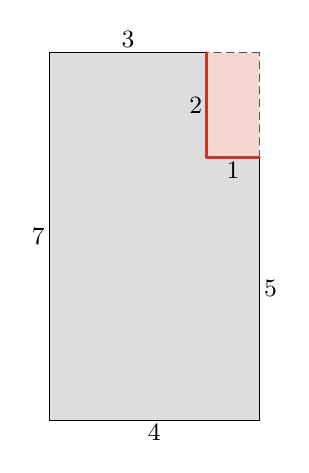
\begin{tikzpicture}
\tkzDefPoint(0.0,0.0){A} %! A = (0, 0)
\tkzDefPoint(2.6666667,0.0){B} %! B = (4, 0)
\tkzDefPoint(2.6666667,3.3333333){C} %! C = (4, 5)
\tkzDefPoint(2.0000000,3.3333333){D} %! D = (3, 5)
\tkzDefPoint(2.0000000,4.6666667){E} %! E = (3, 7)
\tkzDefPoint(0.0,4.6666667){F} %! F = (0, 7)
\tkzDefPoint(2.6666667,4.6666667){G} %! G = (4, 7)
%! fact dist(A, B) == 4
%! fact dist(B, C) == 5
%! fact dist(C, D) == 1
%! fact dist(D, E) == 2
%! fact dist(E, F) == 3
%! fact dist(F, A) == 7
%! fact perp(A, B, B, C)
%! fact perp(B, C, C, D)
%! fact perp(C, D, D, E)
%! fact perp(D, E, E, F)
%! fact perp(E, F, F, A)
%! fact area(A, B, G, F) == 28
%! fact area(C, G, E, D) == 2
%! fact area(A, B, C, D, E, F) == 26
\tkzFillPolygon[color=figtint](A,B,C,D,E,F)
\tkzFillPolygon[color=figaccenttint](D,C,G,E)
\tkzDrawSegment[aux](C,G)
\tkzDrawSegment[aux](G,E)
\tkzDrawPolygon(A,B,C,D,E,F)
\tkzDrawSegment[key](C,D)
\tkzDrawSegment[key](D,E)
\tkzLabelSegment[below,len](A,B){$4$}
\tkzLabelSegment[right,len](B,C){$5$}
\tkzLabelSegment[below,len](C,D){$1$}
\tkzLabelSegment[left,len](D,E){$2$}
\tkzLabelSegment[above,len](E,F){$3$}
\tkzLabelSegment[left,len](F,A){$7$}
\end{tikzpicture}
\end{document}
